\section{Ключевые моменты третьего семестра}

\subsection{События и элементарные исходы}

\begin{definition}[Пространство элементарных событий]
    Некоторое пространство элементарных исходов $\omega$ обозначим
    как $\Omega = \{ \omega_1, \omega_2 \dots \omega_n \dots\}$.
\end{definition}

\begin{example}[О игральной кости]
    Обычная игральная кость содержит шесть ребер, на каждой из которых 
    изображены 1, 2, 3, 4, 5 или 6 точек соответственно. В качестве 
    $\Omega = \{\omega_1 \dots \omega_6\}$ обозначим множество элементарных исходов.
\end{example}

\begin{definition}
    Событием $A$ называется любое подмножество множества $\Omega$: 
    $A \subseteq \Omega$. 

    При этом $A = \Omega$ называют достоверным событием, $A = \varnothing $ называют
    невозможным событием.
\end{definition}

\subsection{Необходимые определения и понятия из алгебры}

\begin{definition}[Алгебра над множеством]
    Алгеброй $\mathcal{A}$ над множеством $\Omega$ называют непустую систему подмножеств некоторого множества $\Omega$, 
    замкнутую относительно операций дополнения и объединения, то есть:
    \begin{enumerate}
        \item $A \in \mathcal{A} \Rightarrow \overline{A} \in \mathcal{A}$
        \item $A, B \in \mathcal{A} \Rightarrow A \cup B \in \mathcal{A}$
    \end{enumerate}
    Стоит отметить, что выполнения этих свойств достаточно, чтобы также 
    выполнялись любые из операций $\cup, \setminus , \triangle$
\end{definition}

\begin{definition}[$\sigma$"=алгебра над множеством]
    $\sigma$"=алгеброй $\mathcal{F}$ над множеством $\Omega$ называют непустую систему подмножеств некоторого множества $\Omega$, 
    замкнутую относительно операций дополнения и счетного объединения, то есть:
    \begin{enumerate}
        \item $A \in \mathcal{F} \Rightarrow \overline{A} \in \mathcal{F}$
        \item $A, B \in \mathcal{F} \Rightarrow A \cup B \in \mathcal{F}$
        \item $\displaystyle \bigcup\limits_1^{\infty}A_k \in \mathcal{F} ~\forall {\{A_k\}}_1^\infty \in \mathcal{F}$
    \end{enumerate}
\end{definition}

\begin{definition}[Минимальная $\sigma$"=алгебра]
    Минимальльной $\sigma$"=алгеброй порожденной набором множеств $\mathcal{H}$
    если:
    \begin{enumerate}
        \item $\mathcal{H} \in \mathcal{F}$
        \item Любая другая $\sigma$"=алгебра $\mathcal{F'}$ содержит в себе $\mathcal{F}$.
    \end{enumerate}
    Иными словами, чтобы найти $\sigma$"=алгебру, содержащую заданный набор
    событий, можно рассмотреть все $\sigma$"=алгебры, содержащие набор
    событий и взять их пересечение.
\end{definition}

\begin{definition}[Борелевская $\sigma$"=алгебра]
    Минимальная $\sigma$"=алгебра, содержащая множество $\mathcal{A}$ всех интервалов
    на вещественной прямой, называется борелевской $\sigma$"=алгеброй в $R$ и обозначается
    как $\mathcal{B}(R)$.
\end{definition}

\subsection{Небходимые определения и понятия из теории меры}
Пусть задано множество $X$ с некоторым классом подмножеств $\mathcal{F}$.
    Предполагается, что этот класс является кольцом множеств или алгеброй множеств.
\begin{definition}[Конечно"=аддитивная/счетно"=аддитивная мера множества]
    Назовем функцию $\mu ~:~ \mathcal{F} \rightarrow [0, +\infty)$, если она удовлетворяет
    следующим условиям:
    \begin{enumerate}
        \item $\mu(\varnothing) = 0$.
        \item $ \mu(A + B) = \mu(A) + \mu(B) ~\forall A, B \in \mathcal{F}: A \cap B = \varnothing$.
        
        Добавление к этому условию условия:
        \item $\mu(\bigcup\limits_{i = 1}^{\infty} A_i) = \sum\limits_{i = 1}^{\infty} P(A_i)$
        позволяет назвать меру счетно"=аддитивной ($\sigma$"=аддитивной).
    \end{enumerate}
\end{definition}

Естественным образом определяется вероятностная мера и ее свойства.
\begin{definition}[Вероятностная мера]
    Вероятностной мерой называется функция $P: \mathcal{F} \rightarrow [0, 1]$ такая, что
    \begin{enumerate}
        \item 
        \begin{equation}
            \label{ref1}
            \forall A \in \mathcal{F}: P(A) \ge 0.
        \end{equation}
        \item
        \begin{equation}
            \label{ref2}
            P(\bigcup\limits_{i = 1}^\infty) = \sum\limits_{i = 1}^\infty P(A_i).
        \end{equation}
        \item
        \begin{equation}
            \label{ref3}
            P(\Omega) = 1. 
        \end{equation}
    \end{enumerate}
    Эти свойства также называются аксиомами вероятности в аксиоматике Колмогорова (о которой речь пойдет позже).
\end{definition}

Из аксиом выше вытекают следующие свойства вероятностной меры.
\begin{theorem}[Свойства вероятностной меры]
    Можно выделить следующие свойства:
    \begin{enumerate}
        \item $P(\varnothing) = 0$ 
        \item $P(\overline{A}) = 1 - P(A)$.
        \item $P(A \cup B) = \begin{cases}
        P(A) + P(B) - P(A \cap B) & A \cap B \neq \varnothing \\
        P(A) + P(B)& A \cap B = \varnothing
        \end{cases}$
        \item $A \subseteq B \Rightarrow P(B \setminus A) = P(B) - P(A)$.
        \item $A \subseteq B \Rightarrow P(A) \le P(B)$. 
    \end{enumerate}
\end{theorem}

\begin{definition}[Аксиоматика Колмогорова]
    Если в вероятностном пространстве ($\Omega, \mathcal{F}, P$) 
    $\mathcal{F}$ является алгеброй событий, а для $P$ выполняются аксиомы
    (\ref{ref1}, \ref{ref2}, \ref{ref3}), то такой набор свойств называется
    аксиоматикой Колмогорова.
\end{definition}

\subsection{Интегралы Лебега}
При работе с интегралами в рамках теории вероятностей
мы будем иметь дело исключительно с интегралами Лебега.
На практике зачастую достаточно использовать и 
интеграл Римана, так как из интегрируемости по Риману
следует интегрируемость по Лебегу.
\begin{figure}[H]
    \centering
    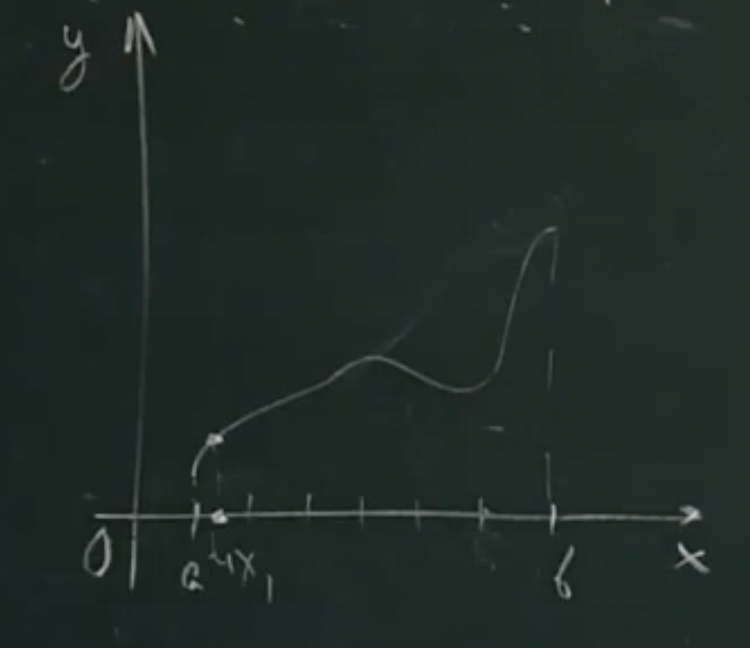
\includegraphics[scale=0.5]{images/riemann.png}
    \caption{Великолепный рисунок, демонстрирующий построение 
    меры Жордана}
\end{figure}

Пусть мы имеем некоторая функцию $f(x)$, определенную на отрезке $[a, b]$.
При работе с интегралами Римана мы строили разбиение $\Delta x_k$ и выберем на каждом $\Delta x_k$
точку $x_k$.
Обозначим как 
$m = \inf\limits_{x \in E} f(x)$, $M = \sup\limits_{x \in E} f(x)$.
Получим
\begin{figure}[H]
    \centering
    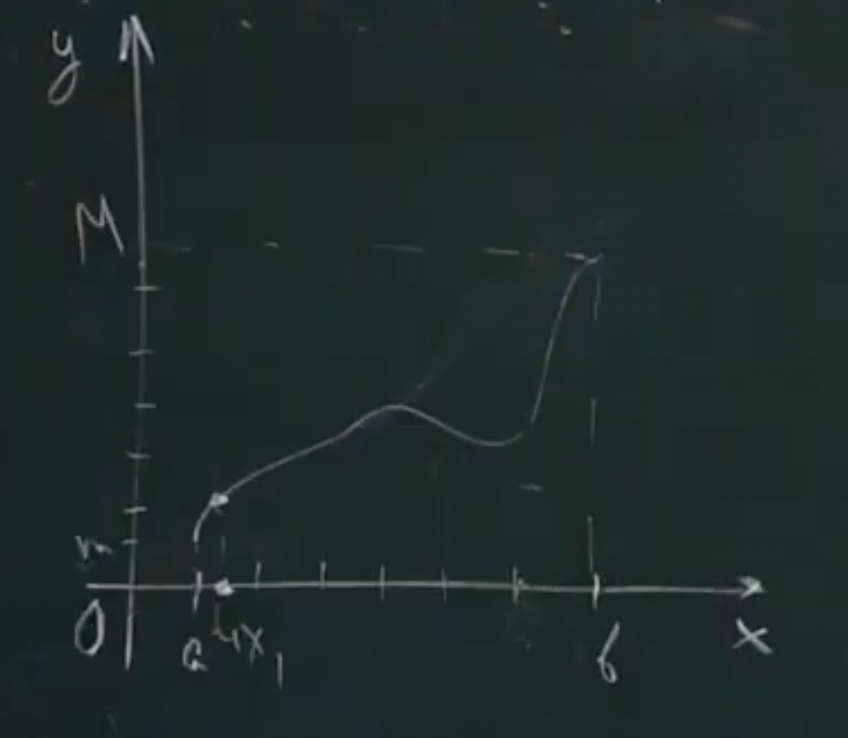
\includegraphics[scale=0.5]{images/lebeg.png}
    \caption{Добавили m и M на Oy}
\end{figure}

Интеграл Лебега, в отличие от интеграла Римана, работает
с разбиениями оси $y$: $E = \coprod\limits_{i = 1}^N E_i$, где

$E_i = \{ x \in E: f(x) \in [y_{i - 1}, y_i]~ \forall i = 1, \dots, N - 1\}$

$E_N = \{x \in E: f(x) \in [y_{N - 1}, y_N]\}$

Получим
\begin{figure}[H]
    \centering
    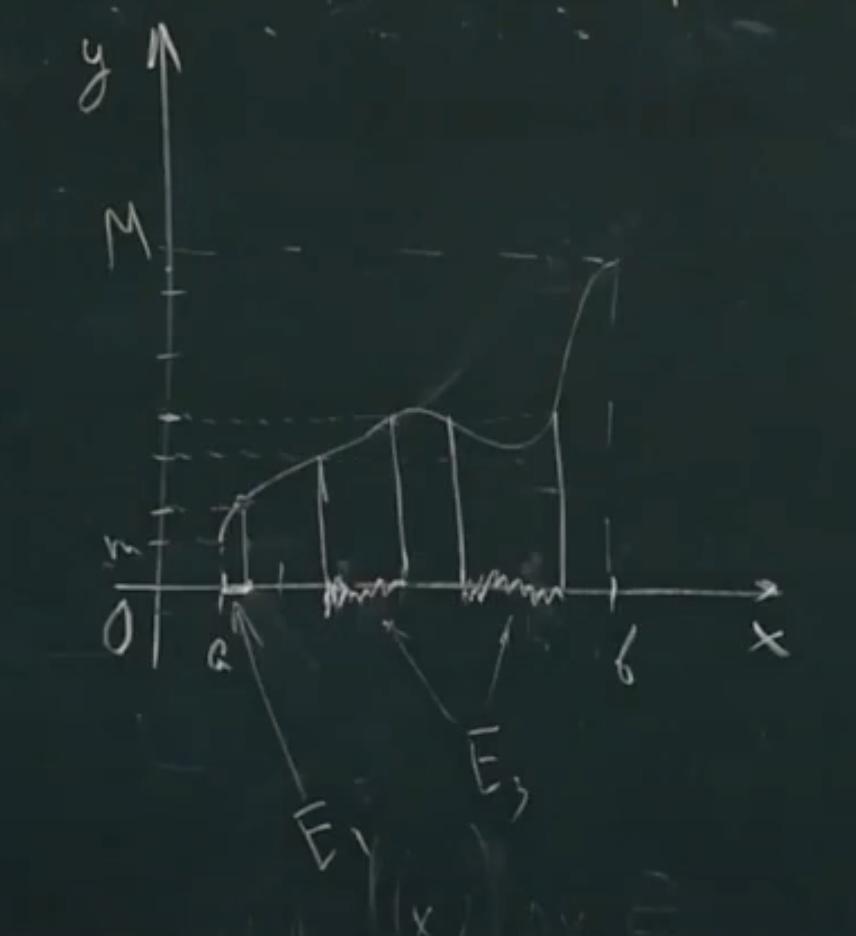
\includegraphics[scale=0.5]{images/lebeg2.png}
    \caption{Построение меры Лебега}
\end{figure}

Обратим внимание, что по большому счету, $E_i = f^{-1}$. то
есть по значению $y$ мы получаем множество точек $x$, попадающих в заданный
интервал разбиения.
\begin{definition}
Внешнюю меру Лебега определим как $m^* E = \inf\left\{\sum\limits_i \Delta_i\right\}$.

При этом внешняя мера любого интервала $[a, b]$ совпадает с его длиной.
        
\end{definition}

\begin{definition}
Внутреннюю меру определим как $m_* E = (b - a) - m^*([a, b] / E)$ для
некоторого отрезка $[a, b]$.    
\end{definition}

Если внутренние и внешние меры равны, то такое множество называются множеством,
измеримым по Лебегу.

\begin{definition}
    Определим интегральные суммы $S = \sum\limits_{k = 1}^n y_k\mu(f^{-1}(\Delta_k)$, 
    $s = \sum\limits_{k = 1}^n y_{k - 1}\mu(f^{-1}(\Delta_k)))$.
    
    Если предел таких сумм существует и они равны между собой, то полученный 
    предел называется интегралом Лебега.
\end{definition}

\subsection{Вероятностные пространства}
\begin{definition}
    Вероятностным пространством называют тройку $(\Omega, \mathcal{F}, P)$ такую,
    что
    \begin{enumerate}
        \item $\Omega$ "--- некоторое множество элементарных исходов
        \item $\mathcal{F}$ "--- $\sigma$"=алгебра подмножеств $\Omega$.
        \item $P$ "--- вероятностная мера, удовлетворяющая аксиомам вероятностной меры.
        \end{enumerate}
\end{definition}
Существует множество вероятностных пространств, среди них выделяют два больших класса.
\begin{definition}
    Вероятностное пространство $(\Omega, \mathcal{F}, P)$ называется дискретным, если
    \begin{enumerate}
        \item $\Omega = \{\omega_1, \omega_2 \dots \omega_n\}$, $n \leq \infty$ (конечно или счетно).
        \item $\mathcal{F} = F_{max}$ (множество всех подмножеств $\Omega$).
        \item $\forall ~ \omega_k, k = 1 \dots N$ задана величина $p_k = P(\omega_k) \geq 0$, при этом
        $\sum\limits_{k = 1}^n p_k = 1$.
    \end{enumerate}
\end{definition}

\begin{definition}
В частности, если $N < \infty, p_k = \frac{1}{n}$, то такое
пространство называют классическим вероятностным пространством.
$P(A)$ в таком случае равно $\frac{M}{N}$, где $M$ "--- число благоприятствующих исходов, $N$ "--- общее число исходов.
\end{definition}

\begin{definition}
    Вероятностное пространство $(\Omega, \mathcal{F}, P)$ называется непрерывным,
    если 
    \begin{enumerate}
        \item $\omega$ "--- некоторая точка пространства.
        \item $\Omega$ "--- область в $n$"=мерном пространстве.
        \item $0 < V(\Omega) = \int\limits_{\Omega}p(x)dx < \infty$.
    
    При этом $p(x)$ "--- некоторая <<весовая>> функция.
    \item $\mathcal{F} = \{A \in \Omega: ~ \exists V(A) = \int\limits_{A}p(x)dx\}$.
    \item  $\displaystyle P(A) = \frac{V(A)}{V(\Omega)}$.
    \end{enumerate}
\end{definition}
\subsection{Условная вероятность и независимость событий}

\begin{definition}
    Условной вероятностью назовем величину $\displaystyle P(A ~|~ B) = \frac{P(A \cap B)}{P(B)}$.
\end{definition}
Условная вероятность позволяет говорить о том, какова вероятность наступления
события $A$, если известно, что событие $B$ наступило.

\begin{theorem}[<<Теорема>> умножения]
    Вероятность того, что оба события произошли одновременно выражаются формулой
    $P(A \cap B) = P(B) P(A ~|~ B)$.
\end{theorem}

\begin{theorem}[Формула полной вероятности]
    Рассмотрим систему событий, имеющих ненулевую вероятность $B_1, B_2, \dots, B_n$, при этом
    $B_i \cap B_j = 0 ~ \forall i \neq j$. Тогда вероятность
    события $A \in \mathcal{F}$, которое может наступить только
    с одним из событий $B_i$ одновременно выражается формулой
    \begin{equation}
        P(A) = \sum\limits_{i = 1}^n P(A ~| B_i) P(B_i)
    \end{equation}
\end{theorem}

Кроме того, нас может интересовать пересчет вероятности наступления
одного из событий $B_i$ при условии, что событие $A$ наступило.
Выразить такую вероятность можно с помощью формулы Байеса.
\begin{theorem}[Формула Байеса]
    Описанная выше вероятность может быть вычислена формулой
    \begin{equation}
        P(B_i ~|~ A) = \frac{P(A ~|~ B_i)P(B_i)}{P(A)}
    \end{equation}
\end{theorem}

\begin{definition}
    События $A$ и $B$ назовем независимыми, если возникновение
    одного из них не влияют на вероятность наступления другого, то
    есть 
    \begin{equation}
        P(A ~|~ B) = P(A), P(B ~|~ A) = P(B) \label{eq:1}
    \end{equation}
\end{definition}
Из последнего неравенство нетрудно получить, так называемый, критерий
независимости событий:
\begin{theorem}[Критерий попарной независимости событий]
    События попарно независимы (или просто независимы), если $P(AB) = P(A)P(B)$.
\end{theorem}
\begin{proof}
    \begin{equation*}
        P(A ~|~ B) = \frac{P(A \cap B)}{P(A)}
    \end{equation*}
    тогда подставляя в (\ref{eq:1}):
    \begin{equation*}
        \frac{P(A \cap B)}{P(A)} = P(B) \Leftrightarrow 
        P(A \cap B) = P(A)P(B)
    \end{equation*}
\end{proof}

\begin{theorem}[О независимости противоположных событий]
    Если независимы события $(A, B)$, то независимы и события $(A, \overline{B})$, $(\overline{A}, B)$, ${(\overline{A}, \overline{B})}$.
\end{theorem}
\begin{proof}
    Для доказательства достаточно рассмотреть независимость применяя критерий независимости.
\end{proof}

\begin{definition}
    События $A_1, A_2, \dots A_n$ называются независимыми в совокупности, если
    для любого подмножества $\displaystyle P(\bigcap\limits_{i = 1}^n) = \prod\limits_{i = 1}^n P(A_i)$ 
\end{definition}

\subsection{Случайные величины}

\begin{definition}
Пусть определены два множества $(X, S_x$) в 
$(Y, S_y)$ с выделенными алгебрами подмножеств и
определена функция $f ~:~ X \rightarrow Y$. Тогда
функция называется $(S_x, S_y)$"=измеримой,
если $\forall y \in Y ~ f^{-1}(y) = x \in S_x$.
\end{definition}
\begin{figure}[H]
    \centering
    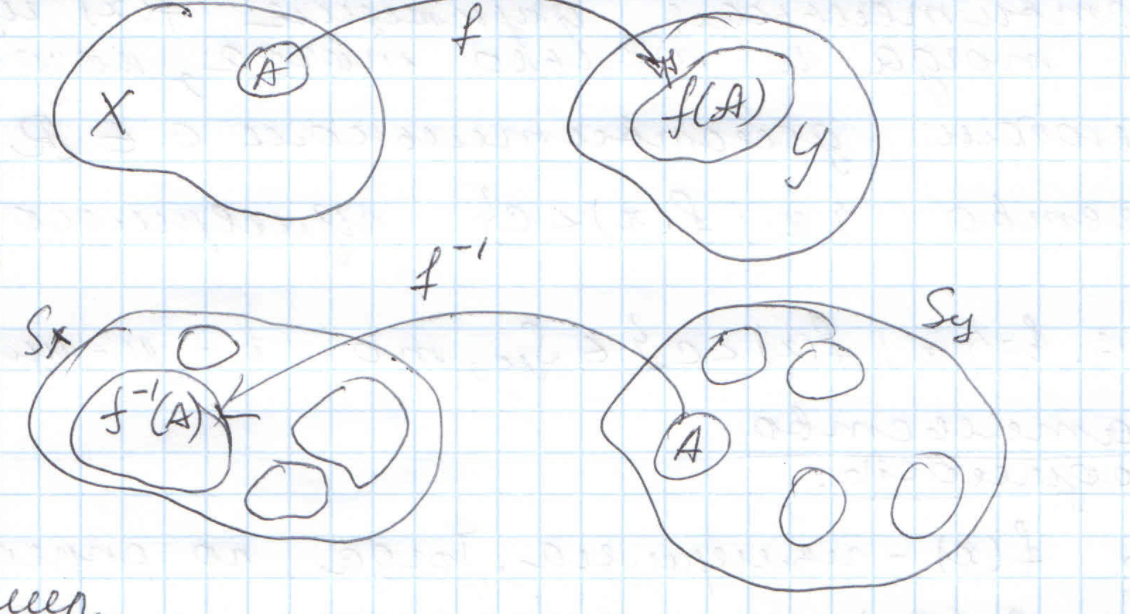
\includegraphics[scale=0.5]{images/izmer.png}
\end{figure}
Если функция вещественнозначная и $S_x = S_y = \mathcal{B}(r)$, то можно
ввести следующее определение:
\begin{definition}
    Действительная функция $f(x)$ на множестве
    $X \subset \mathcal{R}$ называется измеримой, если для любого
    борелевского множества $b$ на числовой прямой $f^{-1}(b) \in S_\mu$(борелевской $\sigma$"=алгебре на $X$).
\end{definition}

\begin{theorem}
    Действительная функция $f(x)$ измерима тогда и только тогда, когда
    при любом $c \in \mathcal{R}$ множество $\{x ~:~ f(x) < c\}$ измеримо.
\end{theorem}

%TODO: Add proof

\begin{definition}
    Определим функцию $\xi ~:~ \Omega \rightarrow \mathcal{R}$ так, что
    $\forall~ x \in R \{\omega ~:~ \xi(\omega) < x\} \in \mathcal{F}$, то есть
    является событием. Такую функцию будем называть случайной величиной.
\end{definition}
Отметим, что исходя из определения эта функция является $(\mathcal{F}, B)$"=измеримой.

\begin{definition}
    Функцией распределения вероятностей случайной величины
    назовем функцию 
    \begin{equation*}
        F(x) = P\{\omega ~:~ \xi(\omega) < x\}    
    \end{equation*}
    Отметим другие формы записи: $F_\xi(x) = P\{\xi < x\}$, $F_\xi(x) = P\{\xi \in (-\infty, x)\}$
\end{definition}

Отметим свойства функции распределения:
\begin{enumerate}
    \item $0 \leq F(x) \leq 1$
    \item $F(x)$ "--- неубывающая, непрерывно слева функция.
    \item $\lim\limits_{x \rightarrow +\infty} F(x) = 1$, $\lim\limits_{x\rightarrow -\infty}F(x) = 0$.
    \item $P\{a \leq \xi < B\} = F(b) - F(a)$
    \item $P\{\xi = x_0\} = F(x_0 + 0) - F(x_0)$
\end{enumerate}
Сразу отметим, что дальнейшие определения отсылают
к определениям дискретного и непрерывного пространства.
\begin{definition}
    Случайная величина называется дискретной, если
    она определена над конечным или счетным множеством значений.
    
    Пусть $\{x_k\}$ "--- допустимые значения случайных величин.
    
    Обозначим как $p_k = P\{\xi = x_k\}$.

    Тогда события $A_k = \{\omega ~:~ \xi(\omega) = x_k\}$ представляют
    из себя полную группу попарно несовместных событий:

    $\bigcup A_k = \Omega$

    $\sum\limits_{i = 1}^\infty p_k = \sum\limits_{k = 1}^\infty P\{ \xi(\omega) = x_k\} = 1$
\end{definition}

Дискретная величина часто задается таблицей, называемой рядом распределения вероятностей.
По такой таблице можно однозначно восстановить функцию распределения.
\begin{definition}
    Законом распределения случайной величины $\xi$ называют
    функцию, по которой вычисляют вероятности значений.
\end{definition}

Функция распределения в дискретном случае представляет из себя
ступенчатую неубывающую функцию 

$F_\xi(x) = \begin{cases}
    0, & x \leq x_1 \\
    p_1, & x_1 < x \leq x_2 \\
    p_1 + p_2, & x_2 < x \leq x_3 \\
    \dots \\
    \sum\limits_{i = 1}^n p_i, & x_{n - 1} < x \leq x_n \\
    \dots \\
    1, & x > x_n
\end{cases}$

\begin{definition}
    Случайная величина $\xi$ называется непрерывной,
    если функция распределения $F(x)$ дифференциируема, то есть:
    $\forall ~ x \in R ~ F(x) = \int\limits_{-\infty}^x dF(t)$ существует.
\end{definition}

\begin{definition}
    Случайная величина $\xi$ называется абсолютно непрерывной, если
    существует такая неотрицательная функция $f(x)$, что
    \begin{equation*}
        \forall ~ x \in R ~ F(x) = \int\limits_{-\infty}^x f(t)dt
    \end{equation*}
    При этом $dF(t) = f(t)dt$, где $f(t)$ "--- плотность распределения.
\end{definition}

\begin{theorem}[Свойства плотности распределения]
    Отметим следующие свойства функции плотности распределения.
    \begin{enumerate}
        \item $f(x) \geq 0$.
        \item $F'(x) = f(x)$ за исключением точек разрыва меры нуль.
        \item $\int\limits_{-\infty}^{\infty}f(x)dx = 1$.
    \end{enumerate}
\end{theorem}

\begin{theorem}[Теорема о существовании сл. в. с заданной ф. р]
    Пусть $F(x)$ "--- неубывающая непрерывная слева функция,
    принимающая значения на отрезке $[0, 1]$. Тогда
    существует дискретное вероятностное пространство $(\Omega, \mathcal{F}, P)$
    и случайная величина $\xi$ на нем, для которой $F(x)$ является
    функцией распределения, то есть 
    \begin{equation*}
    P\{\xi < x\} = F(x)
    \end{equation*}
    Аналогично для абсолютно непрерывного вероятностного пространства.
\end{theorem}

\subsection{Дискретные распределения}
\subsubsection{Распределение Бернулли}
Пусть в пространстве элементарных исходов
эксперимента $\Omega$ рассматриваются только
два события "--- $A, \overline{A}$. Например,
происходит бросок монеты. 

\begin{theorem}[О вероятности, законе и функции распределения]
    В рамках этого распределения определим
    величину $\xi = 0$, если произошла <<неудача>>, то
    есть произошло событие $\overline{A}$ и $\xi = 1$,
    если произошел <<успех>>.
    
    Тогда:
    \begin{enumerate}
        \item Вероятность: $P(A) = p$,
        $P(\overline{A}) = 1 - p = q$.
        \item Закон распределения: $P\{ \xi = k\} = q^{1 - k}p^k$, $k = \{0, 1\}$.
        \item Функция распределения: $F(x) = 
        \begin{cases}
            0, & x \leq 0 \\
            q, & 0 \le x \leq 1 \\
            1, & x > 1 \\
        \end{cases}$
    \end{enumerate}    
\end{theorem}

График распределения:
\begin{figure}[H]
    \centering
    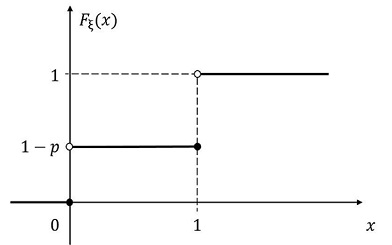
\includegraphics[scale=0.5]{images/bern.jpeg}
    \caption{График функции распределения Бернулли}
\end{figure}

\subsubsection{Биномиальное распределение}
Пусть эксперимент Бернулли повторяется
некоторое число раз. Тогда говорят, что
$\xi$ распределено по $Bin(n, p)$, где
$n$ "--- число испытаний, $p$ "--- вероятность
успеха.

Стохастический эксперимент, в котором возникает
биномиальное распределение называют
<<схемой независимых испытаний Бернулли>>.

%TODO: пример

\begin{theorem}[О законе и функции распределения]
    В рамках этого эксперимента определим
    $\xi \in \{0, 1, \dots n\}$.
    Тогда:
    \begin{enumerate}
        \item Функция вероятности: $P\{\xi = k\} = C_n^k p^k q^{n - k}$
        \item Функция распределения: $F(x) = P\{\xi < x\} = \sum\limits_{k = 0}^x C_n^k p^k q^{n - k}$
    \end{enumerate}
\end{theorem}

График функции вероятности:
\begin{figure}[H]
    \centering
    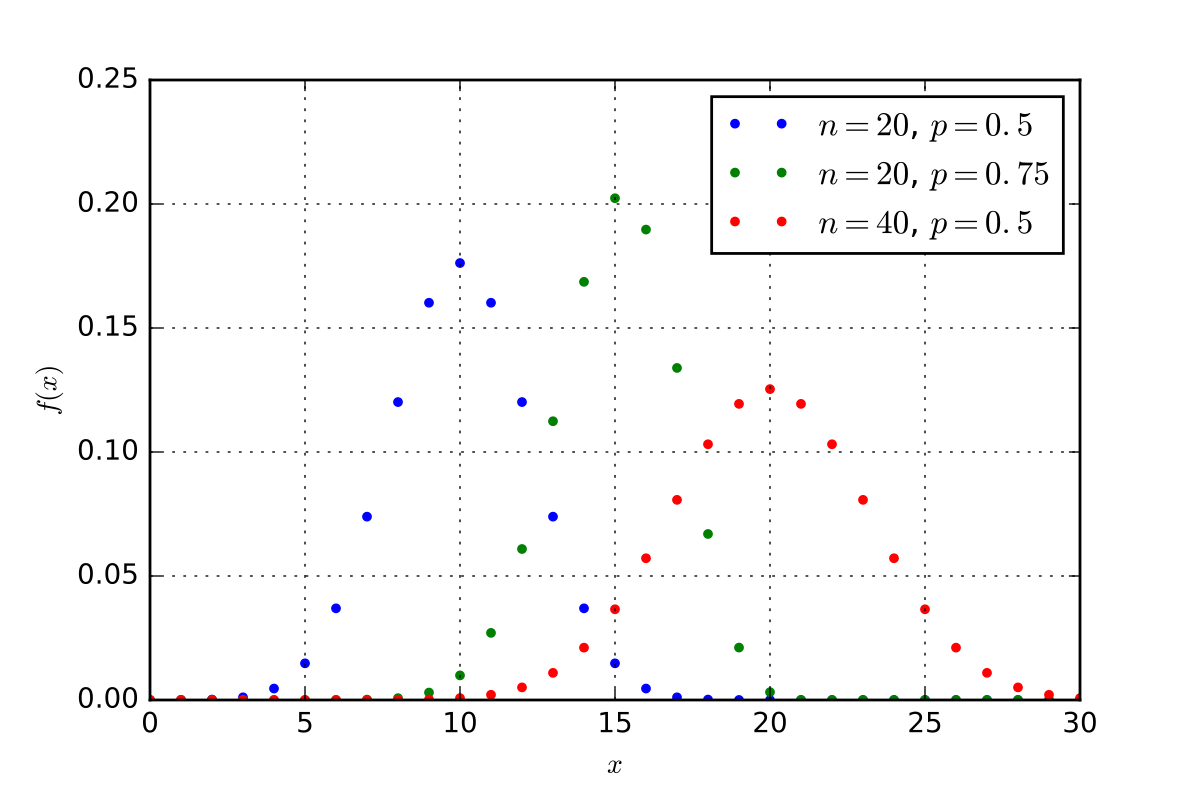
\includegraphics[scale=0.2]{images/binom.png}
    \caption{График функции вероятности}
\end{figure}

График распределения:
\begin{figure}[H]
    \centering
    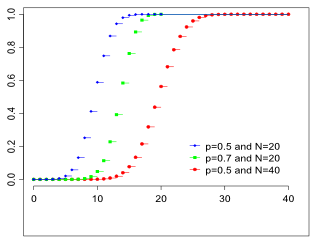
\includegraphics[scale=0.4]{images/binom2.png}
    \caption{График функции распределения}
\end{figure}

\subsection{Распределение Пуассона}
Пусть проводится эксперимент <<по схеме
независимых испытаний Бернулли>>, где
$n$ "--- количество испытаний.

Рассмотрим случайную величину $\xi$ "---
количество <<успехов>> в большом числе
испытаний Бернулли. Тогда математической
моделью такого эксперимента выберем величину
$\xi$ со значениями из множества $\{0, 1, 2 \dots\} \in Z$.

Найдем вероятность $P_n(k) = P(\xi = k)$ "--- того, что
случайная величина $\xi$ примет значение
равное $k$. Так как мы находимся в рамках
схемы Бернулли, то
$P_n(k) = C_n^kp^kq^{n - k}$. Однако, с учетом
множества возможных значений $\xi$ необходимо
совершить предельный переход при $n \rightarrow \infty$.

Тогда
\begin{equation} \label{puas}
    \displaystyle P_n(k) = C_n^k p_n^k q_n^{n - k} = \frac{n!}{k!(n - k)!}p^k q^n q^{-k}
\end{equation}

Пусть $np_n = \lambda_n ~\forall n \in N$, $\lambda_n \rightarrow \lambda$.

Тогда $p_n = \frac{\lambda_n}{n}; q_n = 1 - \frac{\lambda_n}{n}$.

Тогда (\ref{puas}) примет вид:

\begin{equation*}
    \displaystyle 
    \frac{1}{k!} n (n - 1) \dots (n - k + 1) (\frac{\lambda_n}{n})^k(1 - \frac{\lambda_n}{n})^n (1 - \frac{\lambda_n}{n})^{-k} = 
    \frac{\lambda_n^k}{k!} \cdot \frac{n}{n} \cdot \frac{n - 1}{n} \dots \frac{n - k + 1}{n} (1 - \frac{\lambda_n}{n})^{-k} (1 - \frac{\lambda_n}{n})^n)
\end{equation*}

Рассмотрим $\lim\limits_{n \rightarrow \infty}$ полученного выражения.

$\displaystyle \lim\limits_{n \rightarrow \infty}(\frac{n - i}{n}) = 1 - \frac{i}{n} = 1$

Аналогично для $\displaystyle 1 - \frac{\lambda_n}{n}$.

$\displaystyle \lim\limits_{n \rightarrow \infty}(1 - \frac{\lambda_n}{n})^n = e^{-\lambda}$ (второй замечательный предел).

В итоге получим, что $\displaystyle \lim\limits_{n \rightarrow \infty}P_n(k)
 = \frac{e^{-\lambda} \lambda^k}{k!}$.

При этом полученное значение удовлетворяет условию $\sum\limits_{k = 0}^\infty p_k = 1$ (для проверки достаточно
подставить полученное значение под оператор суммы).

Распределением Пуассона называется распределение
случайной величины $\xi$ по описанному выше закону.

$\displaystyle \xi \in N$, $P\{\xi = k\} = \frac{e^{-\lambda} \lambda^k}{k!}$

Функция распределения будет ступенчатой:

\begin{equation*} \displaystyle
    F_\xi(x) = 
    \begin{cases}
        0, & x \leq 0 \\
        e^{-\lambda}, & 0 < x \leq 1 \\
        e^{-\lambda} + e^{-\lambda} \lambda & 1 < x \leq 2 \\
        \dots \\
        \sum\limits_{k = 1}^n \frac{e^{-\lambda} \lambda^k}{k!}
    \end{cases}
\end{equation*}

\begin{figure}[H]
    \centering
    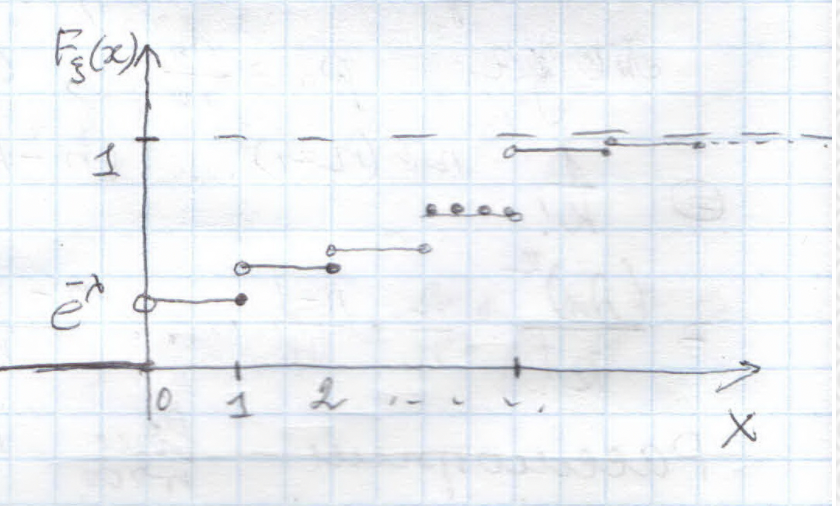
\includegraphics[scale=0.5]{images/puasgraph.png}
    \caption{График распределения Пуассона}
\end{figure}

При этом $\lim\limits_{x \rightarrow \infty} F_\xi(x) = \sum\limits_{i = 1}^\infty \frac{e^{-\lambda} \lambda^k}{k!} = 1$.

\subsection{Геометрическое распределение}

Рассмотрим эксперимент, в котором независимые
испытания Бернулли повторяются до первого
<<успеха>>.

Случайная величина $\xi$ "--- количество экспериментов,
проведенных до появления первого <<успеха>>(включительно).

Распределение этой величины удобно начать с рассмотрения
вероятностного пространства

$\Omega = \{(1), (0, 1), (0, 0, 1) \dots (0, 0, \dots, 1)\}$
при этом постановка эксперимента предполагает, что множество
таких экспериментов счетно.
Тогда $\xi(1) = 1, \xi(2) = 2 \dots \xi(\underbrace{0, 0 \dots 0}_{k - 1}, 1) = k$.

Тогда $P\{\xi = k\} = pq^{k - 1}$.
При этом $\sum\limits_{k = 1}^\infty P\{\xi = k\} = 1$.

\subsection{Равномерное дискретное распределение}

Пусть эксперимент имеет конечное число исходов,
то есть $\Omega = \{\omega_1, \omega_2, \dots, \omega_n\}$.

$P\{w_k\} = \frac{1}{n} ~ \forall i \leq k \leq n$.

Определим случайную величину $\xi$ "--- номер наступившего
исхода.

\begin{figure}[H]
    \centering
    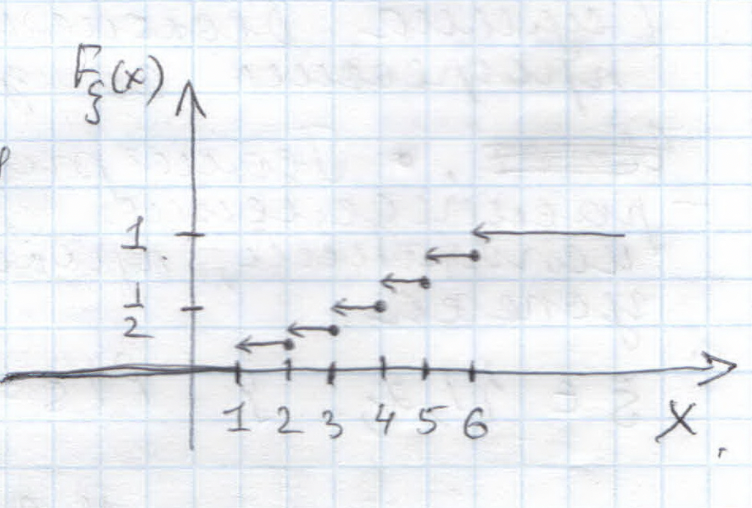
\includegraphics[scale=0.5]{images/ravnomern.png}
\end{figure}

